% !TEX TS-program = pdflatex

\documentclass[border=5pt]{standalone}

\usepackage[utf8]{inputenc}
\usepackage{garamondx}

\usepackage[x11names]{xcolor}

\definecolor{darkolivegreen}{rgb}{0.33, 0.42, 0.18}
\definecolor{darkbyzantium}{rgb}{0.36, 0.22, 0.33}
\definecolor{darkelectricblue}{rgb}{0.33, 0.41, 0.47}
\definecolor{deepchestnut}{rgb}{0.73, 0.31, 0.28}

\usepackage{tikz}
\usetikzlibrary{shapes.geometric, arrows, positioning}

\tikzstyle{required}=[rectangle, rounded corners, minimum width=7em, minimum height=2em, text centered, draw=black, fill=darkolivegreen!30, text width=11em]
\tikzstyle{firstlayer} = [rectangle, rounded corners, minimum width=7em, minimum height=2em, text centered, draw=black, fill=darkbyzantium!30, text width=11em]
\tikzstyle{secondlayer}=[rectangle, rounded corners, minimum width=10em, minimum height=2em, text centered, draw=black, fill=darkelectricblue!30, text width=11em]
\tikzstyle{thirdlayer}=[rectangle, rounded corners, minimum width=7em, minimum height=2em, text centered, draw=black, fill=deepchestnut!30, text width=11em]
\tikzstyle{arrow}=[very thick, ->, >=latex]


\renewcommand{\texttt}[1]{%
  \begingroup
  \ttfamily
  \begingroup\lccode`~=`/\lowercase{\endgroup\def~}{/\discretionary{}{}{}}%
  \begingroup\lccode`~=`[\lowercase{\endgroup\def~}{[\discretionary{}{}{}}%
  \begingroup\lccode`~=`.\lowercase{\endgroup\def~}{.\discretionary{}{}{}}%
  \catcode`/=\active\catcode`[=\active\catcode`.=\active
  \scantokens{#1\noexpand}%
  \endgroup
}

\begin{document}
	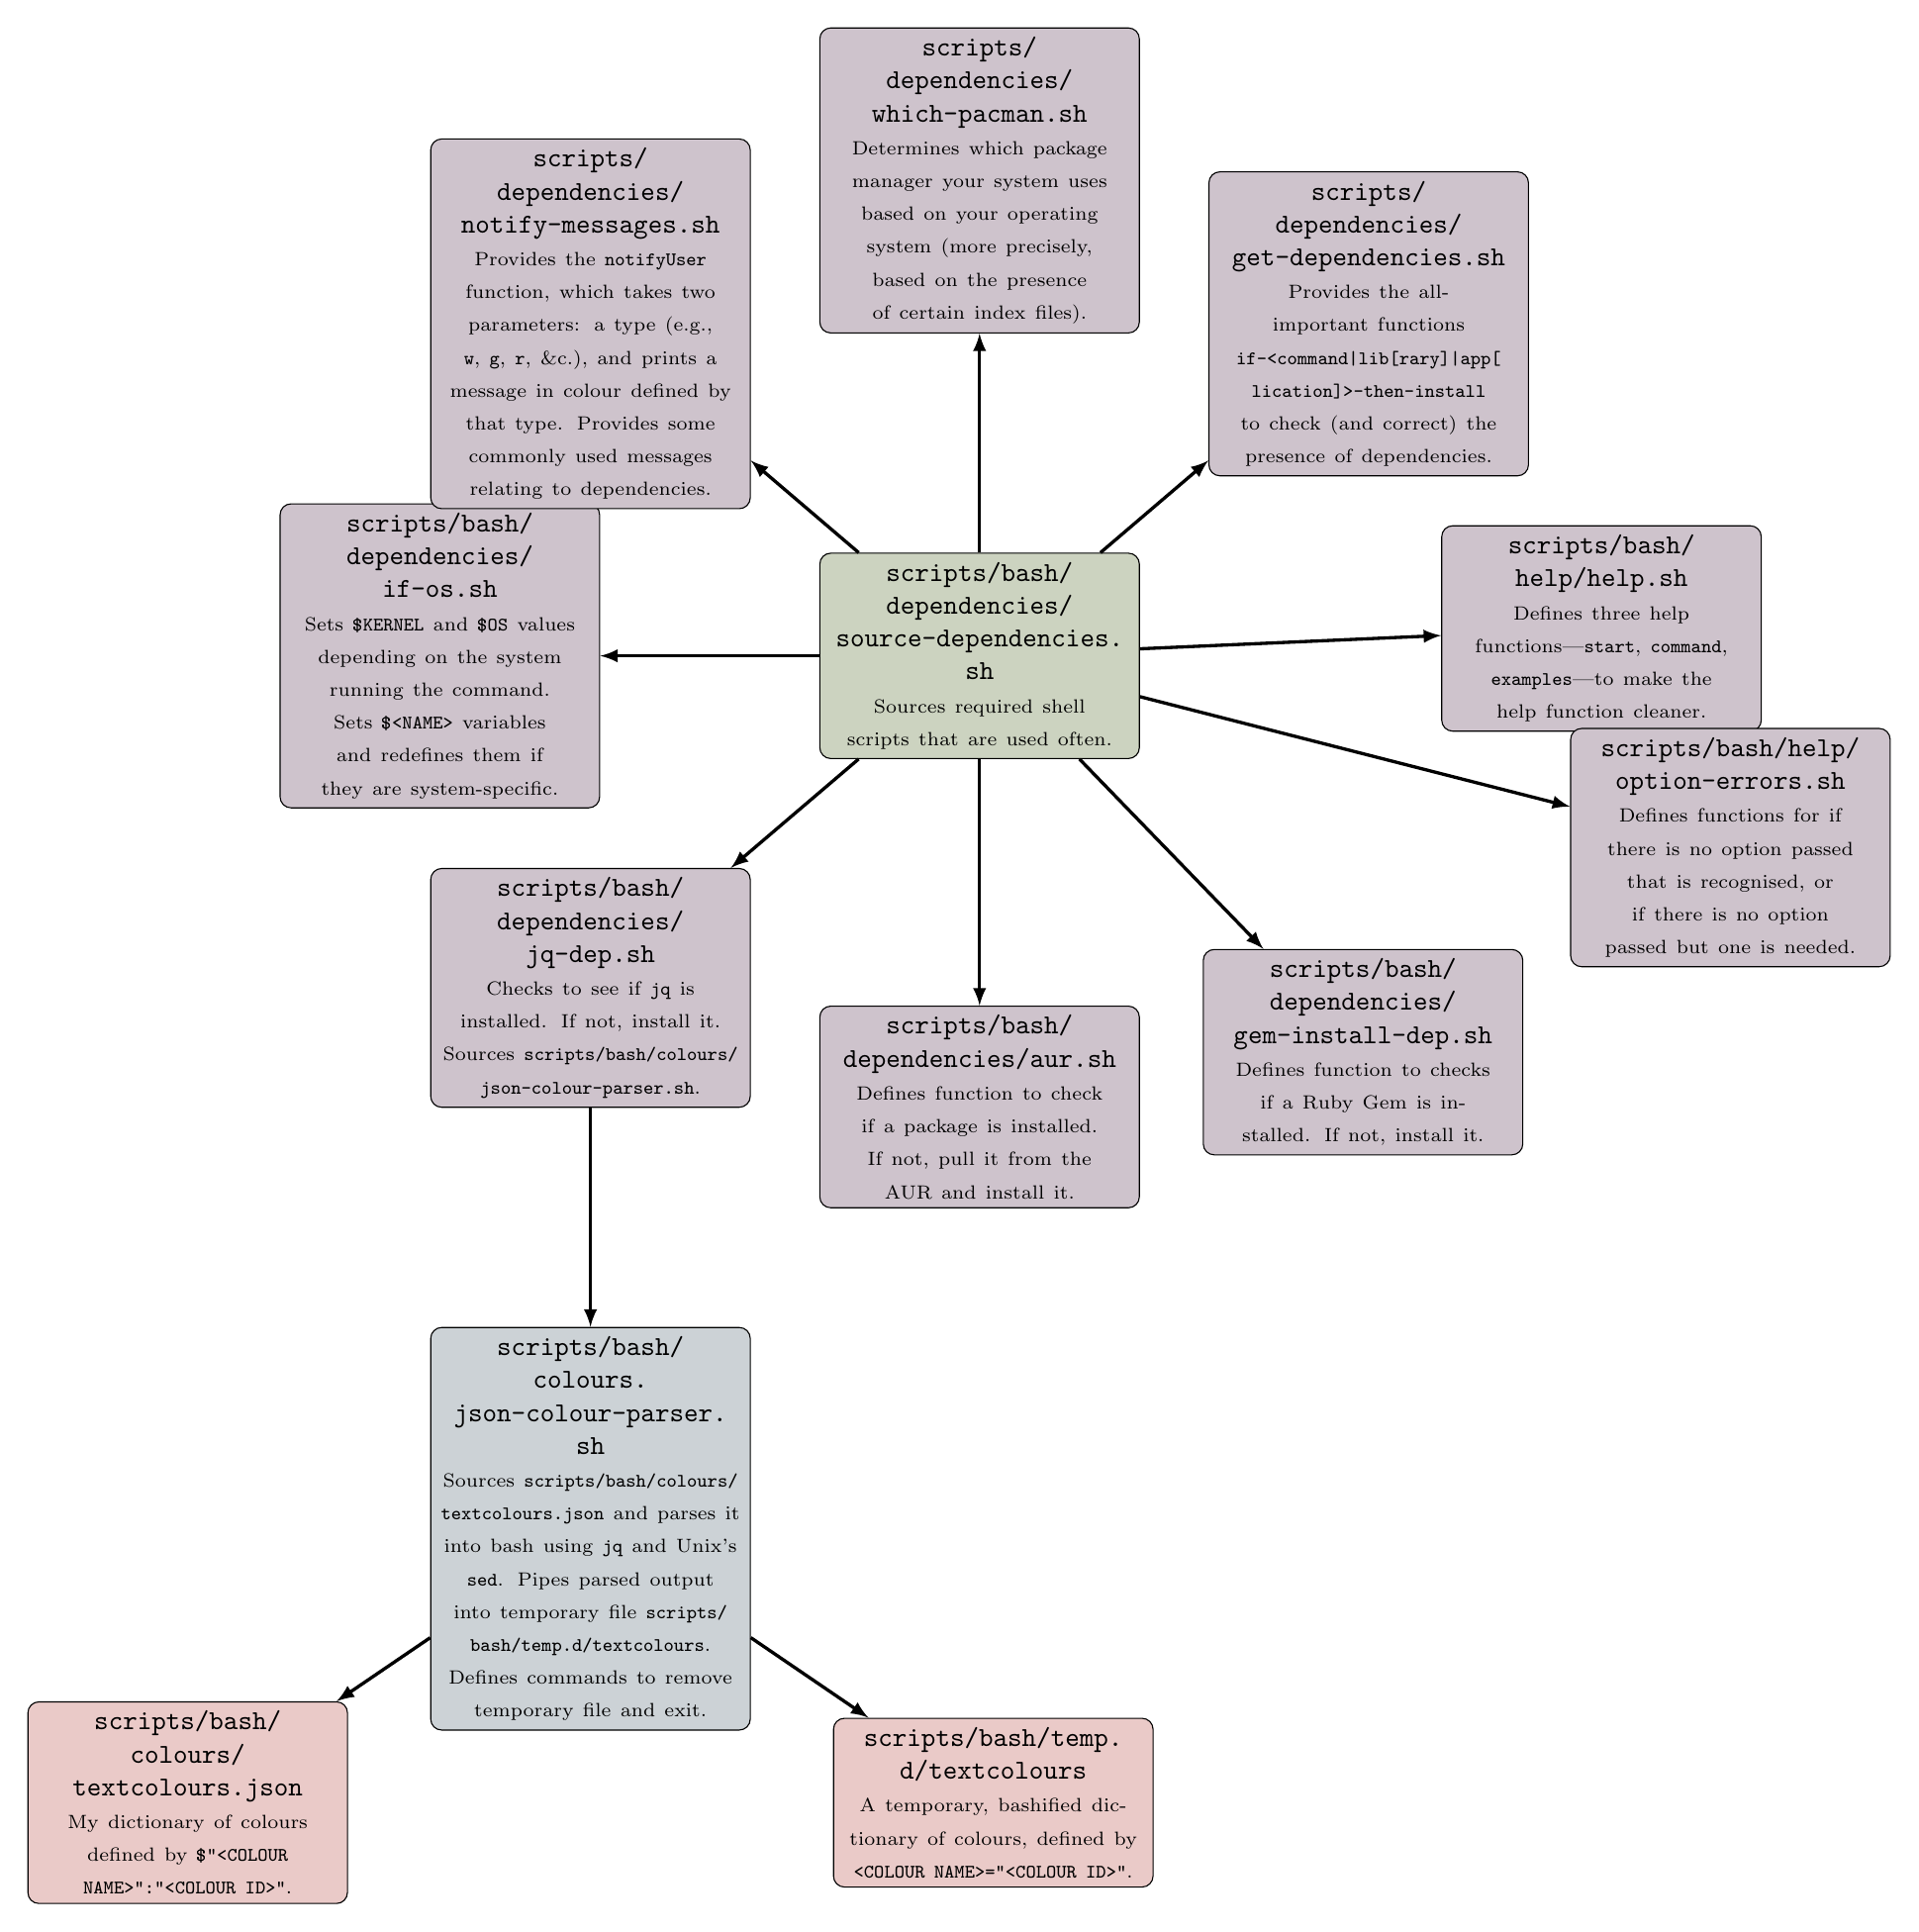
\begin{tikzpicture}[node distance=8em]	
		\node(n1)[required]{\texttt{scripts/bash/dependencies/source-dependencies.sh}\\
		\scriptsize Sources required shell scripts that are used often.};
		
		
		\node(g1)[below=of n1]{};
		
		
		\node(n1-1)[firstlayer, left=of n1]{\texttt{scripts/bash/dependencies/if-os.sh}\\
		\scriptsize Sets \texttt{\$KERNEL} and \texttt{\$OS} values depending on the system running the command.  Sets \texttt{\$<NAME>} variables and redefines them if they are system-specific.};%sources none
		
		
		\node(n1-2)[firstlayer, left=of g1]{\texttt{scripts/bash/dependencies/jq-dep.sh}\\
		\scriptsize Checks to see if \texttt{jq} is installed.  If not, install it.  Sources \texttt{scripts/bash/colours/json-colour-parser.sh}.};%sources dependencies/package-man.sh; sources colours/json-colour-parser.sh
		
		
%		\node(n1-3)[firstlayer, below=of n1]{\texttt{scripts/bash/dependencies/is-command.sh}\\
%		\scriptsize sources \texttt{scripts/bash/dependencies/brew-install-dep.sh}.  Defines function to see if command, library, or application is installed, and to install it if not already installed.};%sources dependencies/brew-install-dep.sh
		
		
		\node(n1-4)[firstlayer, below=of n1, xshift=0em, yshift=-1em]{\texttt{scripts/bash/dependencies/aur.sh}\\
		\scriptsize Defines function to check if a package is installed.  If not, pull it from the AUR and install it.};
		
		
		\node(n1-5)[firstlayer, right of=n1-4, xshift=6em, yshift=2em]{\texttt{scripts/bash/dependencies/gem-install-dep.sh}\\
		\scriptsize Defines function to checks if a Ruby Gem is installed.  If not, install it.};
		
		
		\node(n1-6)[firstlayer, right=of n1, yshift=1em, xshift=3em]{\texttt{scripts/bash/help/help.sh}\\
		\scriptsize Defines three help functions---\texttt{start}, \texttt{command}, \texttt{examples}---to make the help function cleaner.};
		
		
		\node(n1-7)[firstlayer, right=of n1-6, yshift=-8em, xshift=-15em]{\texttt{scripts/bash/help/option-errors.sh}\\
		\scriptsize Defines functions for if there is no option passed that is recognised, or if there is no option passed but one is needed.};
		
		\node(g2)[below=of n1-2]{};
%		\node(n1-2-1)[secondlayer, left=of g2]{\texttt{scripts/bash/dependencies/package-man.sh}\\
%		\scriptsize Defines search and install commands for packages, libraries, and applications, depending on your system.};


		\node(n1-2-2)[secondlayer, below=of n1-2, yshift=0em]{\texttt{scripts/bash/colours.json-colour-parser.sh}\\
		\scriptsize Sources \texttt{scripts/bash/colours/textcolours.json} and parses it into bash using \texttt{jq} and Unix's \texttt{sed}.  Pipes parsed output into temporary file \texttt{scripts/bash/temp.d/textcolours}.  Defines commands to remove temporary file and exit.};
		
		
		\node(n1-2-2-1)[thirdlayer, left=of n1-2-2, yshift=-10em, xshift=5em]{\texttt{scripts/bash/colours/textcolours.json}\\
		\scriptsize My dictionary of colours defined by \texttt{\$"<COLOUR NAME>":"<COLOUR ID>"}.};
		
		
		\node(n1-2-2-2)[thirdlayer, right=of n1-2-2, yshift=-10em, xshift=-5em]{\texttt{scripts/bash/temp.d/textcolours}\\
		\scriptsize A temporary, bashified dictionary of colours, defined by \texttt{<COLOUR NAME>="<COLOUR ID>"}.};
		
		
		\node(g3)[above=of n1]{};
		
		\node(n3-1)[firstlayer,left=of g3]{\texttt{scripts/dependencies/notify-messages.sh}\\
		\scriptsize Provides the \texttt{notifyUser} function, which takes two parameters: a type (e.g., \texttt{w}, \texttt{g}, \texttt{r}, \&c.), and prints a message in colour defined by that type.  Provides some commonly used messages relating to dependencies.};
		
		
		\node(n3-2)[firstlayer,above=of n1]{\texttt{scripts/dependencies/which-pacman.sh}\\
		\scriptsize Determines which package manager your system uses based on your operating system (more precisely, based on the presence of certain index files).};
		
		
		\node(n3-3)[firstlayer,right=of g3]{\texttt{scripts/dependencies/get-dependencies.sh}\\
		\scriptsize Provides the all-important functions \texttt{if-<command|lib[rary]|app[lication]>-then-install} to check (and correct) the presence of dependencies.};
		
		
		\draw[arrow](n1)--(n1-1);
		\draw[arrow](n1)--(n1-2);
%		\draw[arrow](n1)--(n1-3);
		\draw[arrow](n1)--(n1-4);
		\draw[arrow](n1)--(n1-5);
		\draw[arrow](n1)--(n1-6);
		\draw[arrow](n1)--(n1-7);
%		\draw[arrow](n1-2)--(n1-2-1);
		\draw[arrow](n1-2)--(n1-2-2);
		\draw[arrow](n1-2-2)--(n1-2-2-1);
		\draw[arrow](n1-2-2)--(n1-2-2-2);
		\draw[arrow](n1)--(n3-1);
		\draw[arrow](n1)--(n3-2);
		\draw[arrow](n1)--(n3-3);
		
	\end{tikzpicture}
\end{document}